\documentclass[template.tex]{subfiles}
\usepackage{comment} 

\begin{document}

 %% \ SECTION 3
\section{Use cases}

\begin{comment}

Andrew Comments:

Structure: just go through it, Use Case I, Use Case II, Use Case II. No Methods & Results Section

go through it from front to back, explain what an NPZD model is.
"We recreate the NPZD model formulation by Anderson, in the model there is one .." describe equations in words. Then say See Anderson et al. or appendix X for full equations


%  quickly explain overview, explain methods for all of them shortly, with schematics, and put full system of equations & parameter tables in the Appendix!

TODO b4 handing in 2 esteban:
- fix the legend missing in NPZDslab Figure

\end{comment}

% PARAGRAPH STARTS HERE:
To showcase the utility of the phydra package for modelling marine ecosystems, we demonstrate three model implementations of varying complexity.
All model structures present highly idealised versions of marine ecosystems.\\

Use case 1 is a canonical NPZD ecosystem model embedded in a 'slab' physical setting. The specific implementation is adapted from the elegant EMPOWER model \citep{Anderson2015c}, with simplifications to the formulation of light-limited growth of phytoplankton.

Use case 2 presents a more complex size-structured food web embedded in a simple flow-through (chemostat) setting. It is a NPZ model that resolves many size-classes of phytoplankton and zooplankton and their trophic interaction. The model structure was inspired and adapted from \citet{Banas2011b}. 

Use case 3 embeds the complex food web of the second use case within the 'slab' physical setting of the first. Components and processes of each previous model instance are easily combined within the xarray-simlab framework, creating a completely different model, that shows oscillatory inter-annual fluctuations reminiscent of natural plankton populations. \\


The phydra package was designed specifically to create models of flexible dimensionality, as described in Section 2. For the presented use cases we focus on the dimension of ecosystem complexity in relatively simple zero-dimensional physical settings. Models can be run in one, two or three-dimensional physical schemes, by providing the appropriate setup grid and processes defining physical interactions between grid points. Our choice of zero-dimensional implementations was motivated by the fact that such physical schemes are much easier to set up and analyse. The online documentation of the phydra package provides simple examples of multi-dimensional marine ecosystem models.\\



% in final version, present: - jupyter notebook for each example, add links in text

\subsection{Forcing and verification data} \label{ForcingSection}

To simplify models of complex systems larger processes are not mechanistically implemented, but instead empirically represented as an external forcing. In two of the following use cases, we adapt a slab representation of ocean physics as defined by \citet{Evans1985ACycles}. The multi-dimensional ocean is reduced to two layers, where the upper layer provides a zero dimensional setting for our ecosystem model. The bottom layer is often assumed to contain a fixed concentration of nutrients (usually nitrate), but this can also vary with depth or time. There is constant exchange between the layers. Nutrients are usually mixing up into the upper layer, where they are consumed by phytoplankton. 

The fraction of all ecosystem components sinking to the bottom layer are lost from the system. These exchanges of water masses within this two-layered model ocean are driven by the empirically derived mixed layer depth (MLD). Additional common forcings that are used in slab models modify phytoplankton growth, e.g. metabolic rates and light harvesting via temperature and irradiance respectively. Such forcing can situate a slab model in a theoretical or any location in the global ocean. Compared to the natural habitat of marine plankton, the slab model is a radical simplification, however the resulting simulations can yield meaningful results that can be compared with bulk properties of the marine ecosystem. 

\subsubsection{Global nutrient, light and temperature climatologies as slab model forcing}
In line with the concept of phydra as a tool for rapid prototyping of marine ecosystem models, we provide with the package a set of global climatological model forcings. These forcings are derived from satellite data, World Ocean Atlas (WOA) 2018 data and a global MLD climatology kindly provided by Clément de Boyer Montégut.

WOA data provides objectively analyzed climatological mean depth profiles of nutrients (nitrate, phosphate \& silicate) and temperature on a one-degree longitude/latitude grid \cite{Garcia2019WORLDSilicate}. The values have been interpolated from data collected in the World Ocean Database and provide an empirical estimate of the biogeochemical conditions in areas of the global ocean throughout the year.\\

The MLD climatology is an updated version of the original climatology presented in  \citet{deBoyerMontegut2004MixedClimatology}, collecting data up until 2014 and with a modified criterion for MLD. Spatial resolution of the climotology is on a 2 \unit{°} longitude/latitude grid. The analysis of profile data combines a fixed threshold criterion for temperature (0.2 \unit{°C}) and a variable threshold criterion in density (equivalent to a 0.2 \unit{°C} decrease). MLD is diagnosed as the minimum calculated depth of both criterion for each station. This ensures that both temperature and salinity are homogeneous within the mixed layer, and compensated or barrier layers do not skew the values of MLD. This combined MLD criterion corresponds to a proxy of overturning extent depth over a few days, which lends this MLD value very well as the forcing that drives the upwelling of deeper nutrients into the upper mixed layer in slab physics (Clément de Boyer Montégut, personal communication).\\

In addition to the oceanographic and biogeochemical parameters, the provided set of global forcings includes a global climatology of irradiance from satellite data. The NASA satellite MODIS-aqua provides the most up-to-date global climatologies of photosynthetically active radiation (PAR) \cite{MODIS-Aqua2018NASAGroup}. The data product estimates incident PAR at the ocean surface using ..., which can be used to calculate light-availability to phytoplankton within the modelled upper layer.\\

By combining satellite PAR, MLD climatology and WOA data, we can experimentally run a slab model built in phydra in (almost) any location of the ocean. MLD can be used as an empirical forcing for mixing in our slab models. Average nutrient concentration below the mixed layer, extracted from the WOA 2018 climatologies, can be used to provide a more realistic estimate of nutrient supply at certain locations throughout the year. This was done using ... and taking into account 50 \unit{m} below closest available climatological MLD value. The final 1 \unit{°} gridded data product can be accessed via Github [provide link] and is easily integrated with models built using the phydra package. 

From this global forcing dataset, we chose two representative locations in the Atlantic ocean (see Figure \ref{phydraforcing}). These two locations were chosen for their contrasting environment. Temperate with deep MLD in winter, light and temperature variable. Tropical relatively stable conditions throughout the year, lower nutrient supply through mixing. \\


\subsubsection{Satellite chlorophyll and nutrient climatologies as verification data}
Model verification is a very difficult process
- it usually takes specific tailoring of the model to the data, or vice versa \citep{Schartau2017}
- a good fit, does not mean a correct model \citep{RykielJr1996}\\

BUT, still is a basic test of model function, and for demonstration purposes.
We chose to use the Nutrient data from the WOA climatologies for nutrient concentration in the upper layer.

Additionally, we use chlorophyll climatologies from MODIS-aqua (cite!) and 

carbon-based phytoplankton size classes calculated from ocean color estimates of the particle size distribution \cite{Kostadinov2016Carbon-basedDistribution}.\\

The provided dataset provides an easy way to compare model output to empirical data. 

The data are highly aggregated climatologies, of poor temporal resolution (monthly). We follow this path to provide a universally useful, simple tool for marine ecosystem model development. For more specific model implementation and hypothesis testing it would be highly recommended to use local data.\\





\subsection{Use case 1}

The specific NPZD slab model implementation for our Use Case 1 was adapted from \citet{Anderson2015c}. For a schematic of the model structure, see Figure \ref{phydraschematics_1} (a). 
For the full set of equations, please see the Appendix.

\subsubsection{NPZD slab model}
The model contains the name-defining four ecosystem components: Nutrient, phytoplankton, zooplankton and detritus. The only resolved nutrient in this system is nitrate. The biomass of all other state variables is measured in the common model currency \unit{µM} of Nitrogen. Four forcings affect the model dynamics: nitrate below the mixed layer ($N_0$), depth of the mixed layer (MLD), photosynthetically active incident radiation (PAR), average temperature above the mixed layer depth (\unit{T_{MLD}}). The forcings are interpolated monthly climatologies as described in Section \ref{ForcingSection}. See Figure \ref{phydraforcing} for the two locations and specific forcings applied here.\\

% Nutrient dynamics
$N_0$ determines the possible nutrient supply to the ecosystem. Mixing of nutrients is a function of a constant mixing parameter, $N_0$, $N$ and the value and derivative of $MLD$, following \citet{Evans1985ACycles}. In contrast to other components, mixing affecting the nutrient is a positive term adding to $N$ along the gradient between $N_0$and $N$. The general direction of transport is from a nutrient-rich bottom layer to the upper layer supporting phytoplankton growth.

In slab models, the concentration of nutrient in the bottom layer $N_0$ is often assumed to be fixed. In the ocean there is usually a gradient of concentration over depth and this can be represented using functions of nutrient over depth \citep{Frost1987GrazingSpp., Fasham1995VariationsAnalysis}. In this study we use an empirical climatology as the forcing $N_0$, that is the result of combining WOA 2018 data with MLD climatology (see Section \ref{ForcingSection}). The specific variable used is Nitrate+Nitrite. This data provides the contrasting seasonal dynamics for the temperate and tropical location (see Figure \ref{phydraforcing}).

The derivative of MLD affects mixing only when the mixed layer depth is increasing, as 
The change in depth of the mixed layer, described by the derivative of MLD, provides an estimate of mixing intensity. When MLD is shallowing (negative), the loss of component concentration is balanced with the increasing concentration due to a decreasing model volume. A deepening MLD dilutes all components and drives the mixing of nutrient into the upper layer. \\

% Phytoplankton dynamics
The only condition where mixing can bring the nutrient concentration $N$ to approach $N_0$ is when phytoplankton growth is severely limited. In the model, growth of phytoplankton is modified by three factors: Temperature, nutrient uptake and light harvesting. Multiplied by the maximum intrinsic growth rate $\mu_P$ and the current phytoplankton biomass, the growth flux is computed. Temperature dependence of phytoplankton growth is calculated as the Eppley constant \citep{Eppley1972TemperatureSea}, with an exponential equivalent to a $Q_{10}$ of 1.895.
In slab model simulations with a seasonally deep mixed layer, the most limiting factor during these events is often the light-dependence of phytoplankton growth. The light-limiting term is calculated via Steele's formulation \citep{Steele1962EnvironmentalSea}. Incident irradiance is supplied by the PAR climatological forcing. Integrated light availability in the upper layer is calculated via Beer's law, dependent on MLD and the sum of extinction coefficients of water and phytoplankton biomass. Phytoplankton light limitation is further defined by an $I_{opt}$ parameter, that describes what amount of available light saturates photosynthesis, which equals phytoplankton growth in this simplified model.
When sufficient light is available, phytoplankton will consume nutrients. All nutrients consumed are directly incorporated into biomass. This uptake/growth rate is defined by a Monod (or Michaelis-Menten) function, showing a saturating behaviour at high nutrient availability. The maximum rate is defined by the half-saturation constant $k_N$. 
% here phytoplankton mortalities
Phytoplankton mortality is usually implemented as a linear rate, but we follow the EMPOWER model in resolving an additional non-linear term. A linear term describes the effects of natural mortality and metabolic loss. The added quadratic mortality represents density-dependent loss processes, such as virus induced mortalities \citep{Anderson2015c}.  
% note: EMPOWER goes into much greater detail, and cites more publications to support this.
All phytoplankton non-grazing losses contribute to detritus.\\

% Zooplankton dynamics
In this simple model, zooplankton is not affected by environmental factors such as light or temperature. We assume that zooplankton can actively maintain themselves in the upper mixed layer and only compute diluting effects of MLD deepening, but no other mixing terms. 
Zooplankton grazing is the main top-down control of the phytoplankton population in our model. We follow the EMPOWER model in the choice of implementing a multiple-prey grazing formulation acting on both phytoplankton and detritus. In contrast to the grazing formulations employed by e.g. \cite{Fasham1990a}, \citeauthor{Anderson2015c} used a passive switching response, also described as a sigmoidal or Holling type 3 grazing function. The benefit of this type of grazing function over active-switching formulations is that grazing is generally proportional to food availability and the density dependence of prey preference is directly related to single prey responses \citep{Gentleman2003a}.
The specific preferences for phytoplankton and detritus are set at 0.67 for phytoplankton and 0.33 for detritus. This dimensionless prey preference results in a specific half-saturation constant for each prey item, after scaling by the parameter $k_Z$. The actual prey preference during the simulation is dependent on these half-saturation constants and the current biomass of the prey. Passive switching between prey sources describes that with an increase in detritus less phytoplankton will be consumed, but overall intake still increases with any increase in total prey biomass. 
Only a fraction of the biomass grazed by zooplankton is assimilated to zooplankton biomass. Growth efficiency is a product of the absorption efficiency $\beta$ and net production efficiency $k_{NZ}$. Using these two parameters, grazed biomass is split three ways into the fraction actually assimilated to zooplankton, a fraction that is egested to detritus (e.g. faecal pellets) and another that is directly excreted as nutrient. 

Similar to phytoplankton, zooplankton mortality is split into a linear term and a quadratic term. The linear term describes the natural mortality of zooplankton, that is added to the pool of detritus. The quadratic term represents the influence of higher trophic levels that are not further resolved in our zero-dimensional model. This predation-related mortality of zooplankton is assumed to be exported and lost from the system.
This term is also know as the "closure" term, since it stabilises ecosystem dynamics due to the quadratic exponent acting on the highest trophic level.\\

% Detritus dynamics
Detritus is composed of a range of organic material including faecal pellets and aggregates of marine snow of various sizes. In our model we describe an average particle of detrital matter, of which a fraction is remineralised as another fraction is sinking out of the euphotic zone and lost from the system. The processes adding to the pool of detritus are phytoplankton mortality, egested grazing and linear zooplankton mortality. The fraction of detritus that is remineralised each day is given by the parameter $m_D$. In addition to being affected by mixing in the same way as phytoplankton, detritus experiences additional sinking at a rate of $v_D$ (\unit{m \ d^{-1}}).\\

A complete presentation of equations is given in Appendix 1.\\

differences from EMPOWER: \\
Very simple model,
irradiance from satellite, not trigonometric equations. we treat light in much less detail, so say that for a more detailed treatment of light in a slab model, see \cite{Anderson2015c}

Our modifications to phytoplankton growth formulation, zooplankton mixing, as well as the treatment of forcing were adapted from the PhytoSFDM model \cite{Acevedo-Trejos2016}.
% can I say that Esteban? it is true

EMPOWER was inspired by \cite{Fasham1990a}, we stand in a long line of models. 

We hope that this simple NPZD slab model can be used as a teaching model in a similar vein to EMPOWER. The modular structure of phydra processes allows for accessible experimentation with parameterisation and model setup. 


% In EMPOWER i noticed a problem with the shape model output presented in the paper and too large model time steps (due to for loop code structure, not odeint adaptive solving).. is that something I should mention, or simply forget?

\subsubsection{Use case 1 results}
% keep this as dry as possible, just RESULTS no DISCUSSION
Employing the model structure, forcing and parameters presented in the previous sections, exemplary runs were conducted in two contrasting locations. See Figure \ref{NPZDslab_results} for the temporal evolution of the four state variables for the final year of a 5 year run using repeated climatological forcing. 





\subsection{Use Case 2}

From an attempt at describing an oceanic physical setting with a highly simplified ecosystem, we move to a simplified laboratory setting with a complex description of a size-structured ecosystem. This model structure was adapted from \cite{Banas2011b}, with the modification that we explicitly describe the physical setting as a flow-through chemostat. See Figure \ref{phydraschematics_1} (b) for a schematic of the model structure. See Appendix 1.2 for the full system of equations. \\

- Chemostats, a.k.a. continuous cultures, have been regularly used in exploring properties of phytoplankton! Seminal studies of Droop on nutrient uptake were perfomed using chemostats. \citep{Droop1968VitaminLutheri} \\
- also to this day, still an interesting, very simple setting for phytoplankton models\\

Size is called a "master-trait" in the trait-based description of plankton ecology, allowing modellers and ecologist to describe the diverse plankton community along one continuous axis. (This is of course an oversimplification, and it takes careful consideration of the choice of allometries and often a combination of functional properties and size classes to achieve a more realistic representation of natural phytoplankton assemblages.)

\subsubsection{Size-structured NPZ chemostat model}

In comparison to our first use case this model contains only three types of components (namely a nutrient, phytoplankton and zooplankton), but a much larger number of state variables (81 versus 4). The model currency is \unit{\mu M} of Nitrogen, with the only resolved nutrient being dissolved inorganic nitrogen. Additional state variables are 40 size classes of phytoplankton and 40 size classes of zooplankton. These size classes are initialised via a range of equivalent spherical diameters (ESD). For phytoplankton state variables, the ESD determines the nutrient uptake parameters, growth rates and grazing susceptibility, while for zooplankton it sets the prey range, ingestion rates and half-saturation constants of grazing. The specific size-based allometries are taken from meta-analysis of laboratory data (!refs Hansen et al 1997, Hansen et al 1994, Tang 1995, Eppley 1969). 

Thus we can initialise our model with a range of size classes. The size classes are initialised in such a way, that each phytoplankton size class is efficiently grazed by a corresponding zooplankton size class.

Mention how this means:
- there is a "type" or class of component, that uses the same functions, but with varying parameters. This technically corresponds to an array and vectorized computations in python.
- this is what phydra excels at, flexible initialisation of component classes.

%physicalenv
A chemostat is a flow-through system that is often used in laboratories for phytoplankton growth experiments. A population of phytoplankton is inoculated in a bottle, where a constant inflow of nutrients supports their growth. As the volume is kept constant, what flows in must flow out, so a fraction of the volume containing both nutrients and phytoplankton is lost from the system continuously. The balance of nutrient supply, phytoplankton mortality and growth, as well as flow rate defines the trajectory of the system, often towards a steady state at constant flow rates. 
In this model instance, the chemostat provides the zero-dimensional setting for an NPZ ecosystem model. For mechanistic simplicity the detrital pool is not tracked and all detritus is assumed to flow out of the system before being remineralised or grazed upon.

% Nutrient dynamics
The simple physical setting describes two forcing processes, that can be described using a single variable. The chemostat provides an inflow of a nutrient solution, and at the same rate all components are flowing out of the system. The concentration of the external nutrient supply $N_0$ and the flow rate determine the amount of nutrient entering the system over time. The only additional process adding to the nutrient pool within the chemostat is excretion by zooplankton. Other fluxes, such as phytoplankton mortality and zooplankton egestion and mortality, are assumed to be removed from the system.

% Phytoplankton dynamics
Temperature and light are assumed to have no limiting effect on phytoplankton, and therefore dependent processes are not resolved in the model. Phytoplankton growth is only limited by the supply of nutrients. Similar to use case 1, nutrient uptake is instantaneously assimilated to biomass. The growth function for the phytoplankton components is made up of a size-dependent maximum growth rate and a Monod (or Michaelis-Menten) nutrient limiting-term with a size-dependent half-saturation constant multiplied by phytoplankton biomass. 
Phytoplankton losses are the constant outflux, grazing by zooplankton and a general mortality rate, that is a fraction by the size-dependent maximum growth rate $\mu^i_0$. (!ref Moloney and Field, 1991)

% Zooplankton dynamics
Zooplankton grows via assimilating ingested phytoplankton, defined as the product of growth efficiency $\epsilon$ and total ingested phytoplankton. Ingestion of each zooplankton type is a size-dependent process defined by the size of the phytoplankton prey, a half saturation constant $K_s$, the zooplankton type's specific size preference and a size-dependent maximum ingestion rate. [perhaps show a figure visualising the size-dependent allometries?]
The size preference of zooplankton types is assumed to vary with prey size in a log-Gaussian distribution around an optimal prey size for each grazer.
Width of the Gaussian distribution is controlled by the shared prey size tolerance parameter with logarithmic units.
Loss processes of zooplankton are the linear outflux and a quadratic mortality.The quadratic mortality term acts as a closure term, implicitly assuming that the rate of mortality is proportional to total zooplankton biomass (!ref Edwards and Yool, 2000). 
A fraction of grazed phytoplankton biomass, not allocated to assimilation via $\epsilon$ and egestion via $f_{eg}$, is remineralised immediately back into the nutrient state variable.

% allometric parameterisation
The allometric parameterisation follows \cite{Banas2011b}. Values of $\mu^i_0$, $I^j_0$, etc. are determined from power-law functions based on the plankton types ESD taken from review studies [add same table as BANAS 2011?].
- note caveats of allometries
- note the experimental goals of this study


\subsubsection{Use case 2 results}
% JUST RESULTS NO DISCUSSION, moved to SECTION 4
% here explain the ASTroCAT model results
% note that current plot shows ASTroCAT model copy, not the chemostat modification that I have thought up (needs to be implemented and updated)

We present here the results of a 10 year model run using constant forcing in the described chemostat physical setting with one nutrient and 40 size classes of phytoplankton and zooplankton resolved. This corresponds to the base model case presented by \cite{Banas2011b} The major modification is that we moved the model system into a more explicitly theoretical chemostat setting with a constant outflow of model components. 


\subsection{Use Case 3}
In the previous two use cases we presented (1) a NPZD slab model containing 4 state variables within a simplified oceanic physical setting and (2) a NPZ chemostat model containing 81 state variables within a highly simplified laboratory setting. 
In the third use case we want to showcase the highly modular and flexible nature of phydra model components and processes, by placing the highly resolved trophic web of use case 2 within the more realistic physical setting of use case 1.

The resulting model structure is a size-structured NPZD slab model.
- this is already quite a complex model, but there are examples of much more complex models run in global 3D settings in the literature \citep{Ward2012}
- we will compare the model output to size-fractionated phytoplankton biomass (3 size fractions: pico, nano, micro) we group phytoplankton state variables into the three size fractions (See section FORCING for more details)
- for model to data comparison, we need to adjust parameters, do parameter fitting (ideally I'll also do a sensitivity analysis with this model! should be simple using batch dims)

\subsection{Size-structured NPZD slab model}

[This entire section is mostly copied together from the other two, and is quite rough! Still needs some work]\\

For schematic of model structure, see Figure \ref{phydraschematics_3}. Please check appendix for the system of equations. 
Since use case 3 presents no new components or processes from the previous two use case, we will not discuss mechanisms in detail, but highlight from which use case they were adapted where a more detailed description can be found. 

The model contains four ecosystem components: Nutrient, phytoplankton, zooplankton and detritus. The nutrient and detritus component are represented by a single state variable each. Planktonic components of the ecosystem are size-spectrally resolved as in use case 2.
The ecosystem is embedded in a slab physical setting as presented in use case 1. The only resolved nutrient in this system is nitrate. The concentration of all state variables is measured in the common model currency \unit{µM} of Nitrogen. Four external forcings affect the model dynamics: nitrate below the mixed layer ($N_0$), depth of the mixed layer (MLD), photosynthetically active incident radiation (PAR), average temperature above the mixed layer depth (\unit{T_{MLD}}). 

The forcings are the same interpolated monthly climatologies used for use case 1, as described in Section \ref{ForcingSection}. See Figure \ref{phydraforcing} for the two locations and specific forcings applied here.\\

% Phytoplankton dynamics
Growth of phytoplankton is modified by three factors: Temperature, nutrient uptake and light harvesting. Multiplied by the maximum intrinsic growth rate $\mu_P$ and the current phytoplankton biomass, the growth flux is computed. Temperature dependence of phytoplankton growth is calculated as the Eppley constant \citep{Eppley1972TemperatureSea}, with an exponential equivalent to a $Q_{10}$ of 1.895.
The light-limiting term is calculated via Steele's formulation \citep{Steele1962EnvironmentalSea}. Incident irradiance is supplied by the PAR climatological forcing. Integrated light availability in the upper layer is calculated via Beer's law, dependent on MLD and the sum of extinction coefficients of water and phytoplankton biomass. Phytoplankton light limitation is further defined by an $I_{opt}$ parameter, that describes what amount of available light saturates photosynthesis.
The uptake rate of nutrients is defined by a Monod (or Michaelis-Menten) function. The maximum rate is defined by the size-dependent half-saturation constant $k^i_N$. 
% here phytoplankton mortalities
Phytoplankton mortality is implemented as a linear rate, scaled by the size-dependent maximum growth rate. 
All phytoplankton non-grazing losses contribute to detritus.\\

% Zooplankton dynamics
We assume that zooplankton can actively maintain themselves in the upper mixed layer and only compute diluting effects of MLD deepening, but no other mixing terms.
Zooplankton grazing is implemented with the same function described in use case 2 (see Section !3.2!) 

Zooplankton grows via assimilating ingested phytoplankton, defined as the product of growth efficiency $\epsilon$ and total ingested phytoplankton. Ingestion of each zooplankton type is a size-dependent process defined by the size of the phytoplankton prey, a half saturation constant $K_s$, the zooplankton type's specific size preference and a size-dependent maximum ingestion rate. [perhaps show a figure visualising the size-dependent allometries?]
The size preference of zooplankton types is assumed to vary with prey size in a log-Gaussian distribution around an optimal prey size for each grazer.
Width of the Gaussian distribution is controlled by the shared prey size tolerance parameter with logarithmic units.
Loss processes of zooplankton are the linear outflux and a quadratic mortality.The quadratic mortality term acts as a closure term, implicitly assuming that the rate of mortality is proportional to total zooplankton biomass (!ref Edwards and Yool, 2000). 
Only a fraction of the biomass grazed by zooplankton is assimilated to zooplankton biomass. Growth efficiency is a product of the absorption efficiency $\beta$ and net production efficiency $k_{NZ}$. Using these two parameters, grazed biomass is split three ways into the fraction actually assimilated to zooplankton, a fraction that is egested to detritus (e.g. faecal pellets) and another that is directly excreted as nutrient. 

Zooplankton mortality is split into a linear term and a quadratic term. The linear term describes the natural mortality of zooplankton, that is added to the pool of detritus. The quadratic term is assumed to be exported and lost from the system.\\

% Detritus dynamics
The processes adding to the pool of detritus are phytoplankton mortality, egested grazing and linear zooplankton mortality. The fraction of detritus that is remineralised each day is given by the parameter $m_D$. In addition to being affected by mixing in the same way as phytoplankton, detritus experiences additional sinking at a rate of $v_D$ (\unit{m \ d^{-1}}).\\

A complete presentation of equations is given in Appendix 1.\\

\subsubsection{Use case 3 results}
% JUST RESULTS NO DISCUSSION

Using this new complex model structure, and the same forcing used for use case 1, exemplary simulations were performed in two contrasting locations. 
See Figure \ref{SizeStructuredSlab_results} for the average temporal evolution of the aggregated size-classes of \\


- explain here how the runs are set up\\

- explain how the size class comparison works! how do i aggregate the model size classes in the plot\\

- these results will most likely change a lot, once the model & package are re-coded!\\


\clearpage
% Figures

%%f
\begin{figure*}[t]
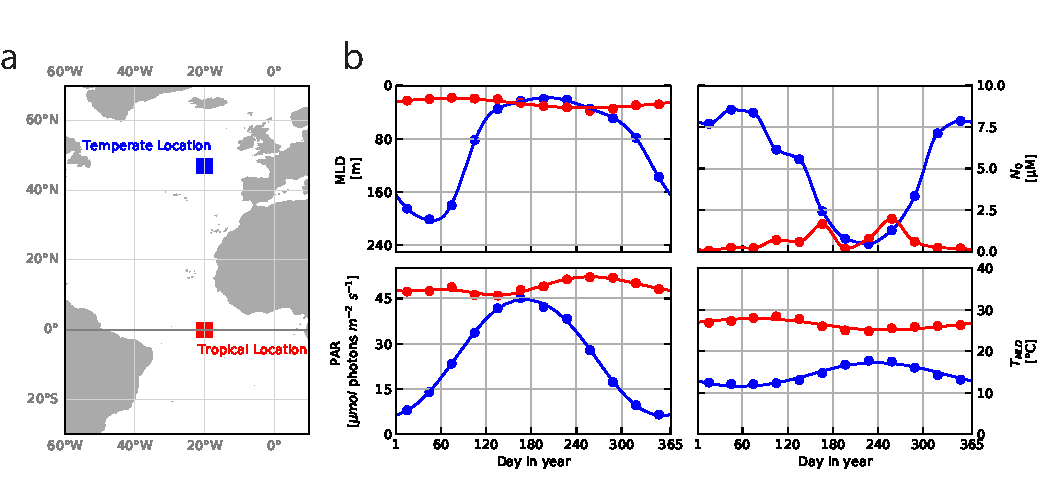
\includegraphics[width=15cm]{Figures/firstdraft_plots/01_forcing_labeled.pdf}
\caption{(a) Map shows locations of the two comparative model runs. Each square is of side length 4° centred on 47°N ,-20°E and 0°N,-20°E respectively. Environmental forcings are averaged across area. (b) Forcing is shown: Mixed Layer Depth (MLD), Nitrate below the Mixed Layer ($N_0$), Photosynthetically Active Radiation (PAR) and temperature averaged across the Mixed Layer ($T_{MLD}$)}
\label{phydraforcing}
\end{figure*}

%%f
\begin{figure*}[t]
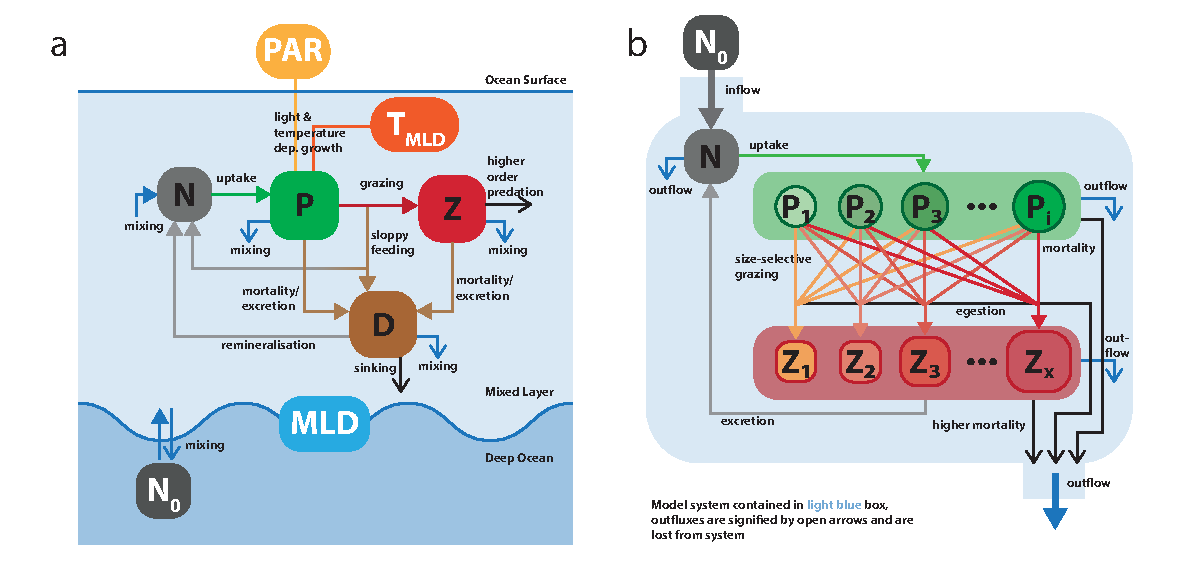
\includegraphics[width=15cm]{Figures/firstdraft_schematics/02__schematics_NPZDandChemostat.pdf}
\caption{(a) Model schematic of NPZD slab model for example 1. Model structure and parameterisation is adapted
from \citet{Anderson2015c} (b) Model schematic of size-structured $NP_{40}Z_{40}$ trophic model for use case 2. Model structure and parameterisation is adapted from \citet{Banas2011b}. [NOTE: these need to be updated, in particular with how egestion and excretion are visualised. Either both originate from grazing flux, or both are originating from "Z".. not this mixture]}
\label{phydraschematics_1}
\end{figure*}


%%f
\begin{figure}[t]
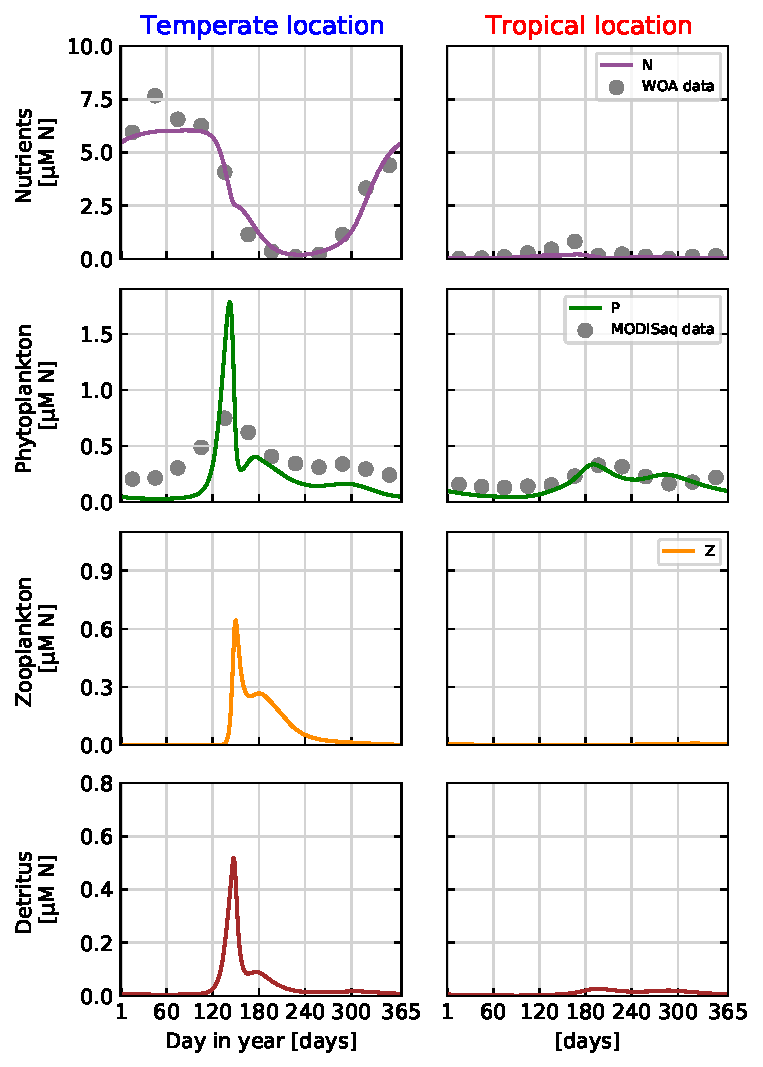
\includegraphics[width=6cm]{Figures/firstdraft_plots/02_NPZDslab.pdf}
\caption{Dynamics of NPZD slab model (i.e. use case 1) in the two exemplary locations. Output is the last year of a 5 year simulation with repeated climatological forcing. Forcing used is shown in Figure \ref{phydraforcing}. Grey dots are verification data from WOA 2018 and satellite climatology (see Section \ref{ForcingSection} for details).}
\label{NPZDslab_results}
\end{figure}

%%f
\begin{figure}[t]
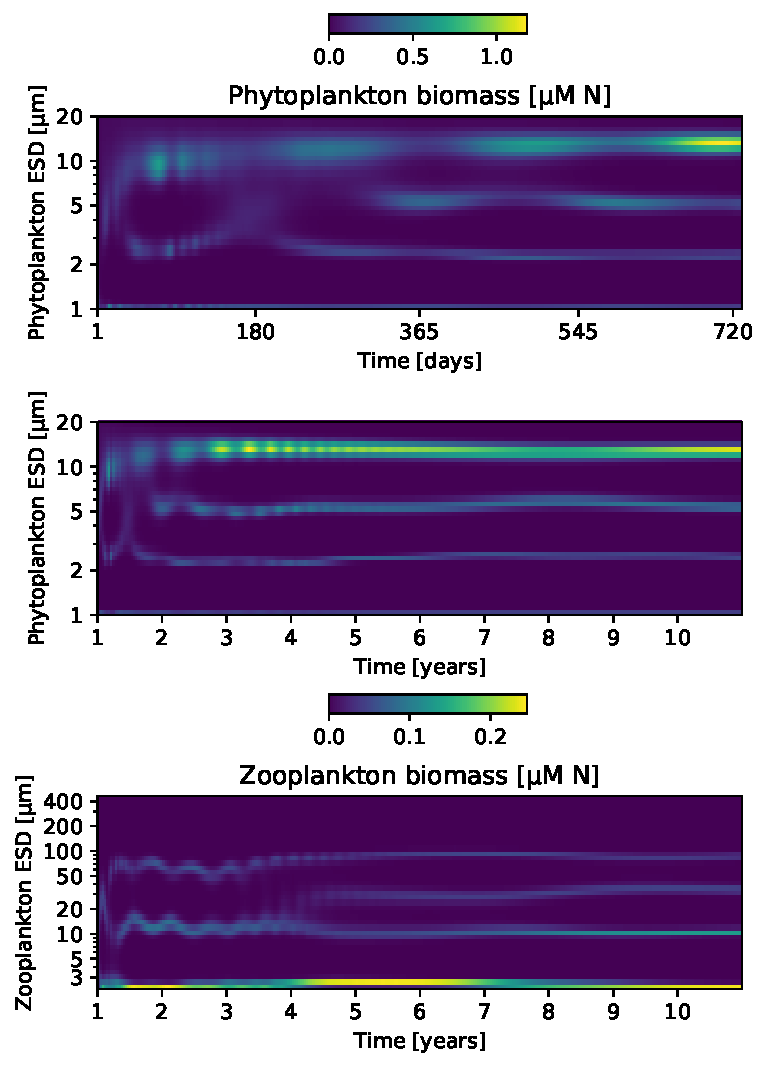
\includegraphics[width=6cm]{Figures/firstdraft_plots/03_chemostat.pdf}
\caption{Phytoplankton and zooplankton biomass per size class under steady chemostat flow-through forcing. Panel (a) shows a detailed view of the first 2 years of simulation. Panel (b) shows 10 years of model time evolution of the same run as the model output approaches a steady state. Panel (c) shows zooplankton biomass time evolution for the same model run. Plot is a recreation (same model setup & parameters) of a plot in \citet{Banas2011b}}
\label{chemostat_plot}
\end{figure}

%%f
\begin{figure*}[t]
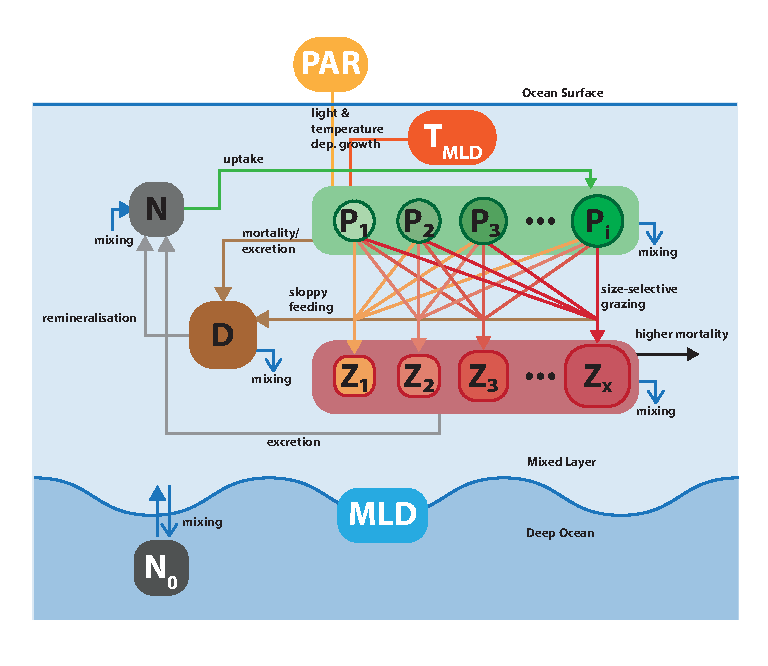
\includegraphics[width=10cm]{Figures/firstdraft_schematics/03__schematics_SizeStructSlab.pdf}
\caption{Model schematic of size-structured \unit{NP_{20}Z_{20}} slab model for use case 3. The model is a combination of the size-structured food web of use case 2 and the detritus component and slab physical setting of use case 1. The model ecosystem is contained in the light-blue area, all open errors represent loss processes that are lost from the system.}
\label{phydraschematics_3}
\end{figure*}



%%f
\begin{figure*}[t]
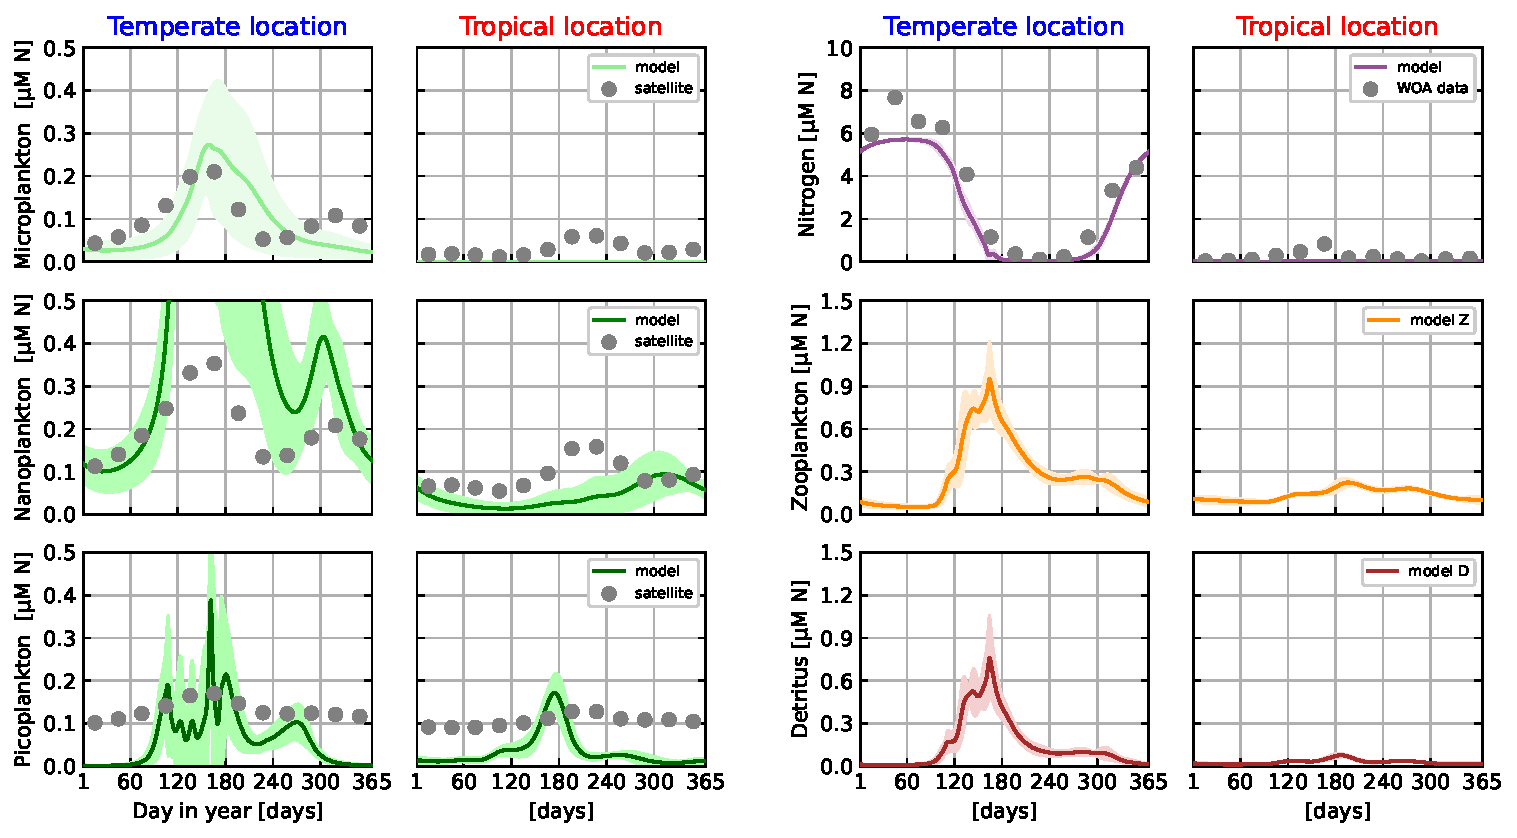
\includegraphics[width=12cm]{Figures/firstdraft_plots/04_sizestruct_slab.pdf}
\caption{Dynamics of size-structured \unit{NP_{20}Z_{20}D} slab model (i.e. use case 3) in the two exemplary locations. Solid line represents the mean dynamics of the last 10 years of a 20 year run with repeated climatological forcing, shaded areas show the standard deviation. Forcing used is shown in Figure \ref{phydraforcing}. Grey dots are verification data from WOA 2018 and satellite climatology (see Section \ref{ForcingSection} for details). Size ranges are picoplankton 0.5 - 2 \unit{\mu m}, nanoplankton 2 - 20 \unit{\mu m}, microplankton 20 - 50 \unit{\mu m}. Zooplankton dynamics shown are the sum of all size classes.}
\label{SizeStructuredSlab_results}
\end{figure*}
% Tables

\clearpage

% this is a custom function to be able to see references when rendering subfiles:
\biblio

\end{document}